\subsection{k-Nearest Neighbors}
\label{section:kNN}

\begin{figure}[t]
    \centering
    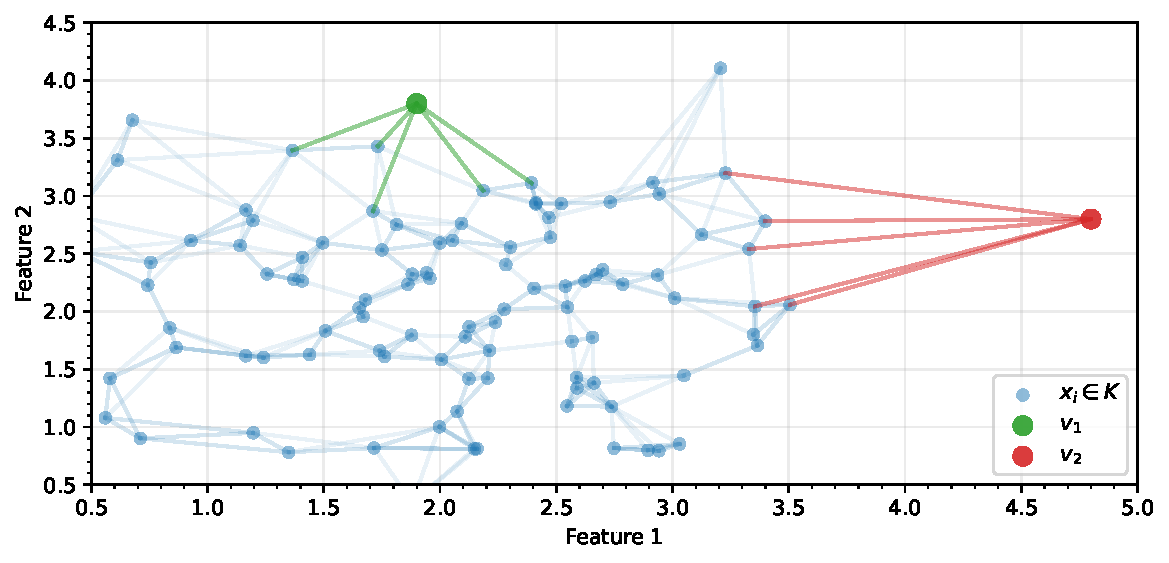
\includegraphics[width=\textwidth]{images/measures/knn-distance.pdf}
    \caption{Idea of the k-Nearest Neighbors applied as an outlierness measure. \\
             The lines drawn connects elements to their $k=5$ closest neighbors.
             Element $v_1$ is~located close to the cluster $T$, so average distance
             to it's closest neighbors is~lower~than for element $v_2$ that is located farther.}
    \label{fig:knn-idea}
\end{figure}

The k-Nearest Neighbors is a well defined, fundamental algorithm of the machine learning~\cite{Hastie-2009}, that is useful in variety of tasks, such as in clusterization and classification. It was recently proposed as a state-of-the-art out-of-distribution detector \cite{Sun-2022}.

The core concept assumes the identification of given $k$ number of elements from a~known set $T$ that are closest neighbors of a given element $v$. Such identification can be performed by using one from a number of possible underlying algorithms, for~example a~naive brute-force search or by utilizing sophisticated data structures, like with k-dimensional tree \cite{Bentley-1975}\cite{Brown-2015} or ball tree algorithm \cite{Omohundro-1989}\cite{Liu-2006}. Also, for distance calculation, there may be any of the known metrics involved, such as the Manhattan/L1 distance or the general Minkowski metric; commonly the standard Euclidean distance is used \cite{Singh-2013}.

In applications for outlier detection, there are two main approaches proposed in the literature. First solution relies on selecting the distance to the $k$-th neighbor as the outlierness score, i.e., the highest distance among all $k$ neighbors around given $v$,
\begin{equation}
    {kNN}_{I}(v, T)
    =
    \max\big\{
        ~
        \forall x_i \in N_k(v, T): ~ \norm{\vv{v - x_i}}
        ~
    \big\}
    ,
    \label{eq:kNN-max}
\end{equation}
where $N_k(v, T)$ is a function that returns the set containing $k$ number of elements $x_i$ from cluster $T$ that are closest to $v$. The second approach relies on calculating the average distance to all of $k$ considered neighbors,
\begin{equation}
    {kNN}_{II}(v, T)
    =
    \frac{1}{k}
    \cdot
    \left(
        ~
        \sum_{x_i \in N_k(v, T)} \norm{\vv{v - x_i}}
        ~
    \right)
    .
    \label{eq:kNN-avg}
\end{equation}

Typically, the high values of the calculated outlierness score, above certain threshold, indicate that given feature vector $v$ is far from all samples present in training cluster $T$, i.e., it is an outlier. Respectively, low values of the score indicate that the $v$ is not distant from known examples, hence it is an inlier.

Figure \ref{fig:knn-idea} illustrates the representation of example cluster $T$ from the kNN algorithm's perspective, along with in-distribution sample ($v_1$) and outlier ($v_2$). The key advantage of the algorithm is that no arbitrary assumption on the data distribution is required, as it relies purely on the proximity of the neighbor points. On the other hand, the algorithm is therefore sensitive to any incorrectly labeled entries in the training dataset that may lead to further spurious assignments.

It shall be noticed that for the very, very large datasets, containing huge number of high-dimensional feature vectors ($n \sim 1\,000\,000\,000$), the process of identifying the nearest neighbors can become slow and the model may be difficult to fit into RAM (Random Access Memory). To~overcome this, companies that deal with searching through such enormous amounts of data on daily basis presented recently their dedicated solutions for this problem. The Faiss library\footnote{\url{https://github.com/facebookresearch/faiss}} \cite{Douze-2024}, developed mainly by Fundamental AI Research group at Meta (formerly Facebook), is an example solution that utilizes the product quantization based approach for approximate nearest neighbor search \cite{Jegou-2011}. Another example is Annoy library\footnote{\url{https://github.com/spotify/annoy}} (Approximate Nearest Neighbors Oh Yeah), developed by Erik Bernhardsson and used at Spotify for music recommendations, that supports file-based indexes mapped into RAM that can be effectively shared between multiple system processes.

During the research the implementation from the scikit-learn library \cite{scikit-learn} was used.
